% ch32-fp4-persist-d.tex — FP4(二)：persist-D 主 kernel 与两级 P 量化（RFC-K6）★
% 源码：ffpa-attn(861d75e) cute/fp4/sm_120/persist_d.cuh(1113L) + fp4_pscale.cuh(793L) + fp4_gemm.cuh(276L)
\chapter{FP4（二）：persist-D 主 Kernel 与两级 P 量化}\label{ch:32}

\section{本章导读}

第~\ref{ch:31}~章把 Q/K/V 送进了 e2m1 + ue4m3 的 workspace；本章讲
消费它们的\textbf{主 kernel}：
\texttt{fp4\_persist\_d\_fwd\_}\allowbreak\texttt{cute\_fp4\_sm120}
（\texttt{sm\_120/persist\_d.cuh}，1113 行），跑在 fp8 persist-D 同款
128 线程 producer + 256 线程 consumer 的 warp-specialized 骨架上
（第~\ref{ch:29}~章），数据路径移植自 SageAttention3 的 NVFP4 kernel。

本章的主角是\textbf{两级 P 量化}——SA3 对「$P$ 无法离线校准」这一挑战
的回答，也是 fp4 attention 精度成立的最后一块拼图。它不是独立的
pass，而是与 online softmax \textbf{融合}在一起的
（\texttt{fp4\_pscale.cuh} 的 \texttt{SoftmaxFused}）：softmax 吐出的
每个数直接落进第二级量化的域，$s_{P1}$ 的常数折进 \texttt{exp2} 的
shift，除法和归一化在到达寄存器之前就已经消失。

\section{问题与动机}

\textbf{P 的三重困境}。Q/K/V 的量化无论多粗，都可以离线统计
（smooth、per-block scale）压动态范围；$P$ 不行：
\begin{enumerate}[itemsep=0pt,topsep=2pt]
  \item \textbf{online}：$P$ 是 softmax 现场产物，kernel 内逐 tile 生成，
        没有第二遍数据；
  \item \textbf{值域窄}：$P\in[0,1]$，且行内分布剧变——causal 早期行
        近 one-hot（一个 1、其余 $\approx0$），dense 行近均匀且数值极小；
  \item \textbf{SF 格式自身的损耗}（SA3 的 C2 挑战）：若按块直接量化，
        $s_P=\mathrm{amax}(P_{块})/6\in[0,0.167]$，ue4m3 在这个窄域的
        有效位数被浪费——\textbf{尺度因子自己}先损失精度，再乘回 16
        个元素。
\end{enumerate}
两级量化的思路：先把整行线性拉伸到 NVFP4 的满量程（第一级，全局
常数），块内再用 e2m1 域归一（第二级，per-16 组 ue4m3）——让块的
$\mathrm{amax}$ 恰好铺满 ue4m3 的域。

\textbf{硬件侧的结构约束}。blockscale MMA
（\texttt{m16n32k64 kind::mxf4nvf4}，\texttt{attn\_traits.cuh} L77）要
求 K 维 64 对齐、SF 以 \texttt{scale\_vec::4X} 旁路喂入；P 作为 A 操作
数必须以 data+SF 的 zip 形式出现（\texttt{fp4\_pscale.cuh} L314--346 的
pack 注释）。这套约束决定了 P 量化必须发生在寄存器里、紧贴 MMA。

\section{数学原理}

\subsection{两级 P 量化：SA3 §3.2 的方案}

对 softmax 输出 $\tilde P$（已减行 max、未归一），两级量化定义为：
\begin{equation}
  s_{P1}[row]=\frac{\mathrm{rowmax}(\tilde P)}{448\times6},\qquad
  \tilde P_2=\frac{\tilde P}{s_{P1}}\in[0,\,2688],\qquad
  \hat P_2,s_{P2}=\phi(\tilde P_2)
  \label{eq:32-two-level}
\end{equation}
$2688=448\times6$：分子是 ue4m3 满量程、分母是 e2m1 满量程，第一级把
行拉伸到「SF 与数据的乘积极限域」。dequant 端
$O=\mathrm{FP4MM}(\hat P_2,s_{P2},\hat V,s_V)\times s_{P1}$，常数
$s_{P1}$ 在 $O$ 与 row\_sum 中\textbf{同现同消}——finalize 相除后精确
抵消（\texttt{fp4\_pscale.cuh} L327--330 注释）。

\subsection{online softmax 下的退化：第一级变成常数}

ffpa 实现的关键洞察（\texttt{fp4\_pscale.cuh} 头注释 L2--5）：online
softmax 对当前 tile 已经减去运行行 max，所以
$\mathrm{rowmax}(\tilde P)\equiv1$，逐行的 $s_{P1}$ \textbf{退化为全
局常数} $1/(448\times6)$，可以直接折进 \texttt{exp2} 的 shift：
\begin{equation}
  P_2=\exp_2\!\bigl(S\cdot L-m\cdot L+\log_2(448\cdot6)\bigr)
  \in[0,\,2688],\qquad
  s_{P2}=\exp_2\!\bigl(a\cdot L-m_{sc}+\log_2\tfrac{1}{6}\bigr)\in(0,\,448]
  \label{eq:32-p2-domain}
\end{equation}
其中 $L=\mathrm{scale}\cdot\log_2 e$，$a$ 是 16 元素组 absmax，$m_{sc}$
是含第一级常数的行 max（L117--119 注释与 L126--128 的三个编译期
常数：$\log_2(1/2688)=-11.3923$、$\log_2(1/6)=-2.5850$）。第一级量化
的除法、$s_{P1}$ 的存储与乘回全部消失。常数符号容易看错：
$m_{sc}=m\cdot L+\log_2\frac{1}{2688}$，减去它等效加上
$\log_2 2688$，所以 $s=m$ 时 $P_2$ 恰达 $2688$（源码注释 L118 把
shift 写作 $+\log_2(1/(448\cdot6))$，是同款符号笔误，以代码与值域为
准）。

\subsection{归一化也折进 exp2}

第二级本需要 $q=\tilde P_2/s_{P2}$（数据除以组尺度才能落 e2m1 域）。
实现把这一步同样折进指数（L182--186 注释）：
\begin{equation}
  q=\exp_2\!\bigl((s-a)\cdot L+\log_2 6\bigr)\in(0,\,6]
\end{equation}
组 absmax 归一化在 \texttt{exp2} 参数里完成，\textbf{rcp 与逐元素
FMUL 在 softmax 与 pack 之间整段消失}；row\_sum 用 FMA 吸收 $s_{P2}$
因子（\texttt{row\_sum = fmaf(q, sfp2, row\_sum)}，L195）。硬件只要
一条 MUFU.EX2——\texttt{ex2.approx.ftz.f32} 的 \texttt{.ftz} 让 ptxas
不必包 range glue（L21--22 注释，非 ftz 形式每次调用要多出 FSETP/
FSEL/FMUL 链，实测 -5.9\%）。

\textbf{同一条 shuffle 链做两个归约}：C fragment 每 lane 持 8 元素，
$\texttt{shfl\_xor}(1)$ 合成 16 元素组 absmax，$\texttt{shfl\_xor}(2)$
完成 quad 内行 max（L160--167）——组尺度和行 max 的冗余
归约减半。

\textbf{全 masked 组的退化}：$a=-\infty$ 时特判 $a\to0$（L187 的
\texttt{a\_arg} clamp），$q$ 与 row\_sum 贡献双双归 0 而不是 NaN；
\texttt{InfCheck} 模板参数处理整行有效列全部落在当前 tile 之外的
causal 左上角（L169--175、L219--221 的 \texttt{scores\_max\_cur} 守卫）。

\subsection{lazy rescale 与 lse 复合公式}

跨 tile 的行 max 更新沿用 fp8 的 lazy rescale（第~\ref{ch:29}~章）：
$O$ 不即时重缩放，记 \texttt{scores\_scale}，下一个 tile 的 PV 累加前
按行补乘（\texttt{rescale\_acc}，L299；PC-11 起为 per-row 守卫——
\texttt{scores\_scale(mi)<1.0f} 的行跳过 FMUL，dense 路径 96.5\% 命中
零开销，\texttt{persist\_d.cuh} L968--975 注释）。

lse 的复合公式（每项都有出处）：
\begin{equation}
  \mathrm{lse}=\bigl(m\cdot L+\log_2(\mathrm{row\_sum})+
  \log_2\tfrac{1}{2688}\bigr)\ln 2+\mathrm{scale}\cdot q_{km}
  \label{eq:32-lse}
\end{equation}
第一项是 log2 域行 max 与 row\_sum，第三项是两级量化的 $1/2688$ 因子
（行和处于 $P\cdot2688$ 域，要除回来），最后一项是 smooth-K 的修正
$\mathrm{dot}(q_{row},\bar k)$（第~\ref{ch:31}~章
式~31-deltas 的对应项；\texttt{lse\_qkm\_dot} 在 Q 寄存器拷贝后、kv
循环之前算好，L583--591 与 \texttt{persist\_d.cuh} L757--758——Q 的
smem 在 \texttt{kQSmemReuse} 下会被 V stage 复用，点积必须提前）。

\subsection{MXFP8 PV 变体的数值契约}

\texttt{--fp4-pv-mm-type fp8} 把 $V^\top$ 换成 e4m3 + ue8m0（32 元素
组），P 侧同样换 32 粒度两级量化：域常量从 2688 换成 $448$（e4m3 满
量程，无第二级 e2m1 因子），SF 是 2 的幂
（\texttt{pow2\_to\_ue8m0}，L417；契约注释 L390--397）。SFA 的槽位排
布按 \texttt{SM120\_16x8x128\_TN\_VS\_MXFP8} atom 的 A 布局走
（L501--535 的 probe 结论）。历史上 MXFP8 PV 的 lse 曾无条件沿用
2688 域——差 $\ln 6$ 的 latent bug，现按 \texttt{kPvMxfp8} 编译期分
流。

\section{设计与实现}

\subsection{骨架复用与 grid 调度契约}

WS 骨架与 fp8 persist-D 同构：128T producer（TMA 装载 K/V/SF/bias）+
256T consumer（8 warp MMA），4 组反向 barrier
（\texttt{k\_empty}/\texttt{v\_empty}/\texttt{q\_consumed}/
\texttt{epilogue\_done}，L200--213 注释）。fp4 特有的协议纪律：所有
mbarrier \textbf{永不 re-initialize}——per-CTA 全局 kv-tile 计数器驱动
每个 barrier 的 stage/phase 跨 work 连续翻转（对活跃 mbarrier 的
re-init 是 UB，PTX ISA 9.7.13.15.9；L113--115、L316 注释）。

grid 调度契约是「\textbf{单 kernel、单代码路径、runtime grid 定风格}」
（L92--120 注释）：kernel 体是
\texttt{for (work\_id = blockIdx.x; work\_id < total\_work; work\_id +=
gridDim.x)} 的 strided work loop。dense 用
$\min(total\_work, SMs)$（persistent，流水 fill/drain 每 CTA 摊一次，
producer 可在 consumer 跑 epilogue 时预取下一个 work 的 K/V）；causal
用 \texttt{total\_work}（经典 block-per-work，短 work 早完早释放 SM，
HW 调度器负载均衡——多数 work 的 $T_{c,eff}\ll T_c$，persistent 的
每 work 固定开销会占主导）。barrier 协议对任意 gridDim 都成立，
non-persistent 只是每 barrier 只翻第一个 phase 的退化情形。

\subsection{Q 的寄存器驻留与一个教科书级 bug}

Q/SFQ 是 per-work 常量：s2r 一次进 \texttt{tSrQ}/\texttt{tSrSFQ} 寄存
器，跨整个 kv 循环驻留，\texttt{gemm\_ss\_fp4} 把它们当 A 侧寄存器操
作数消费、不再每 tile 读 Q smem（L747--753 注释——fp8 的
\texttt{kPersistQs2r} 等价物，这里恒开）。这段注释同时记录了一个值得
抄走的 bug：\textbf{没有}寄存器驻留时，A/SFA 的 asm 操作数未初始化，
cicc 直接把它们折叠成 0，QK 退化成 $\Delta S$（rank-1 均值 attention）
——probe 容差曾把它掩盖。教训：量化 kernel 的「输出恒为常数」类退化
要靠数据探针（输出对 K 的敏感性）而非容差卡。

\subsection{主循环五步}

consumer 的 kv 循环（L803--971）每 tile 依次：
\begin{enumerate}[itemsep=0pt,topsep=2pt]
  \item \texttt{add\_delta\_s}：把 $\Delta S$ 的 rank-1 项预载进 C 累
        加器（只写 \texttt{tSrS} 寄存器，与 B 侧操作数装载无重叠，
        L819--822）；
  \item \texttt{gemm\_ss\_fp4}：$S\mathrel{+}= (\hat Q\,s_Q)(\hat K\,s_K)$。
        A 侧驻留寄存器、B 侧（K/SFK）从当前 stage 流入，操作数是
        data+SF 的 \texttt{make\_zip\_tensor} 对（\texttt{fp4\_gemm.cuh}
        L131--132）；B 的下一个 k\_block 拷贝与当前 mma 交叠发出，链尾
        的 \texttt{k\_empty} arrive 让 producer 恰在 mma 消费完时看到
        stage 释放（L140）；
  \item masking：kv-tail + causal 谓词\textbf{必须}用
        $pos=kv\_tile\cdot B_c+kv\_perm32(j)$（L903--916，谓词在
        L911）；bias 注入
        在 dequant 域（除 \texttt{scale\_orig}），列同样过 $\pi$，tile
        化路径（PC-0-1）持有原始 token 序、注入时索引置换
        （L838--896）；$-\infty$ 赋值同时覆盖 masked 槽位的
        $\Delta S$ 垃圾；
  \item \texttt{online\_softmax\_with\_quant}：32.3 节的融合体，输出
        已在 $P_2$ 域的分数 + \texttt{AbsMaxP} 组尺度；
  \item \texttt{gemm\_rs\_fp4}：$O\mathrel{+}= (\hat P_2\,s_{P2})
        (\hat V\,s_V)$。A（P）不过 smem——\texttt{quantize\_and\_pack\_p}
        刚在寄存器里打包好；V 的 copy、量化、mma 按此顺序发出让 S2R
        与 mma 链重叠，链尾 \texttt{v\_empty} arrive 兼作「无更多预取」
        分支（\texttt{fp4\_gemm.cuh} L171--180 注释）。
\end{enumerate}
V 的 \texttt{v\_full} 等待放在 softmax \textbf{之后}（L937--940）：
QK 数学与 V 的 TMA 传输重叠。slot 轮转按 work 内 tile 索引、barrier
按全局序列（\texttt{v\_slot}/\texttt{v\_mem} 解耦，L811--814），
\texttt{kQSmemReuse} 下 V 的 slot 0 别名到 Q 区，轮转避开别名区
（\texttt{attn\_traits.cuh} L62--65）。

\subsection{epilogue：finalize、加回与批量 staging}

循环后 \texttt{finalize} 除以 row\_sum（0 行守卫）；smooth-V 的
$v_m$ 逐列加回（恒等推导见 \texttt{persist\_d.cuh} L981--1016 的完整
注释——softmax 权重和为 1，$v_m$ 对所有列相同，从列和里提出后与
归一化相消；masked 列 $P=0$ 不参与两个和，causal 下恒等式同样成立）。
然后是 O 的批量 staging：consumer named barrier（WAR fence，确认所有
PV 读与 lse dot 完成）$\to$ \texttt{SM90\_U32x2\_STSM\_N} 把
\texttt{tCrOHalf} 写进 SW128 smem（叠在被释放的 Q/K 区上）$\to$
单条 TMA store（L1018--1066）。tail Q tile 走 R$\to$G 带行守卫。
注意 STSM 用 \texttt{U32x2} 而非 fp8 的 \texttt{U32x4}——blockscale
PV 的 C fragment 每 lane 持数不同（头注释 L44--46）。

\section{图示}

\begin{figure}[H]
  \centering
  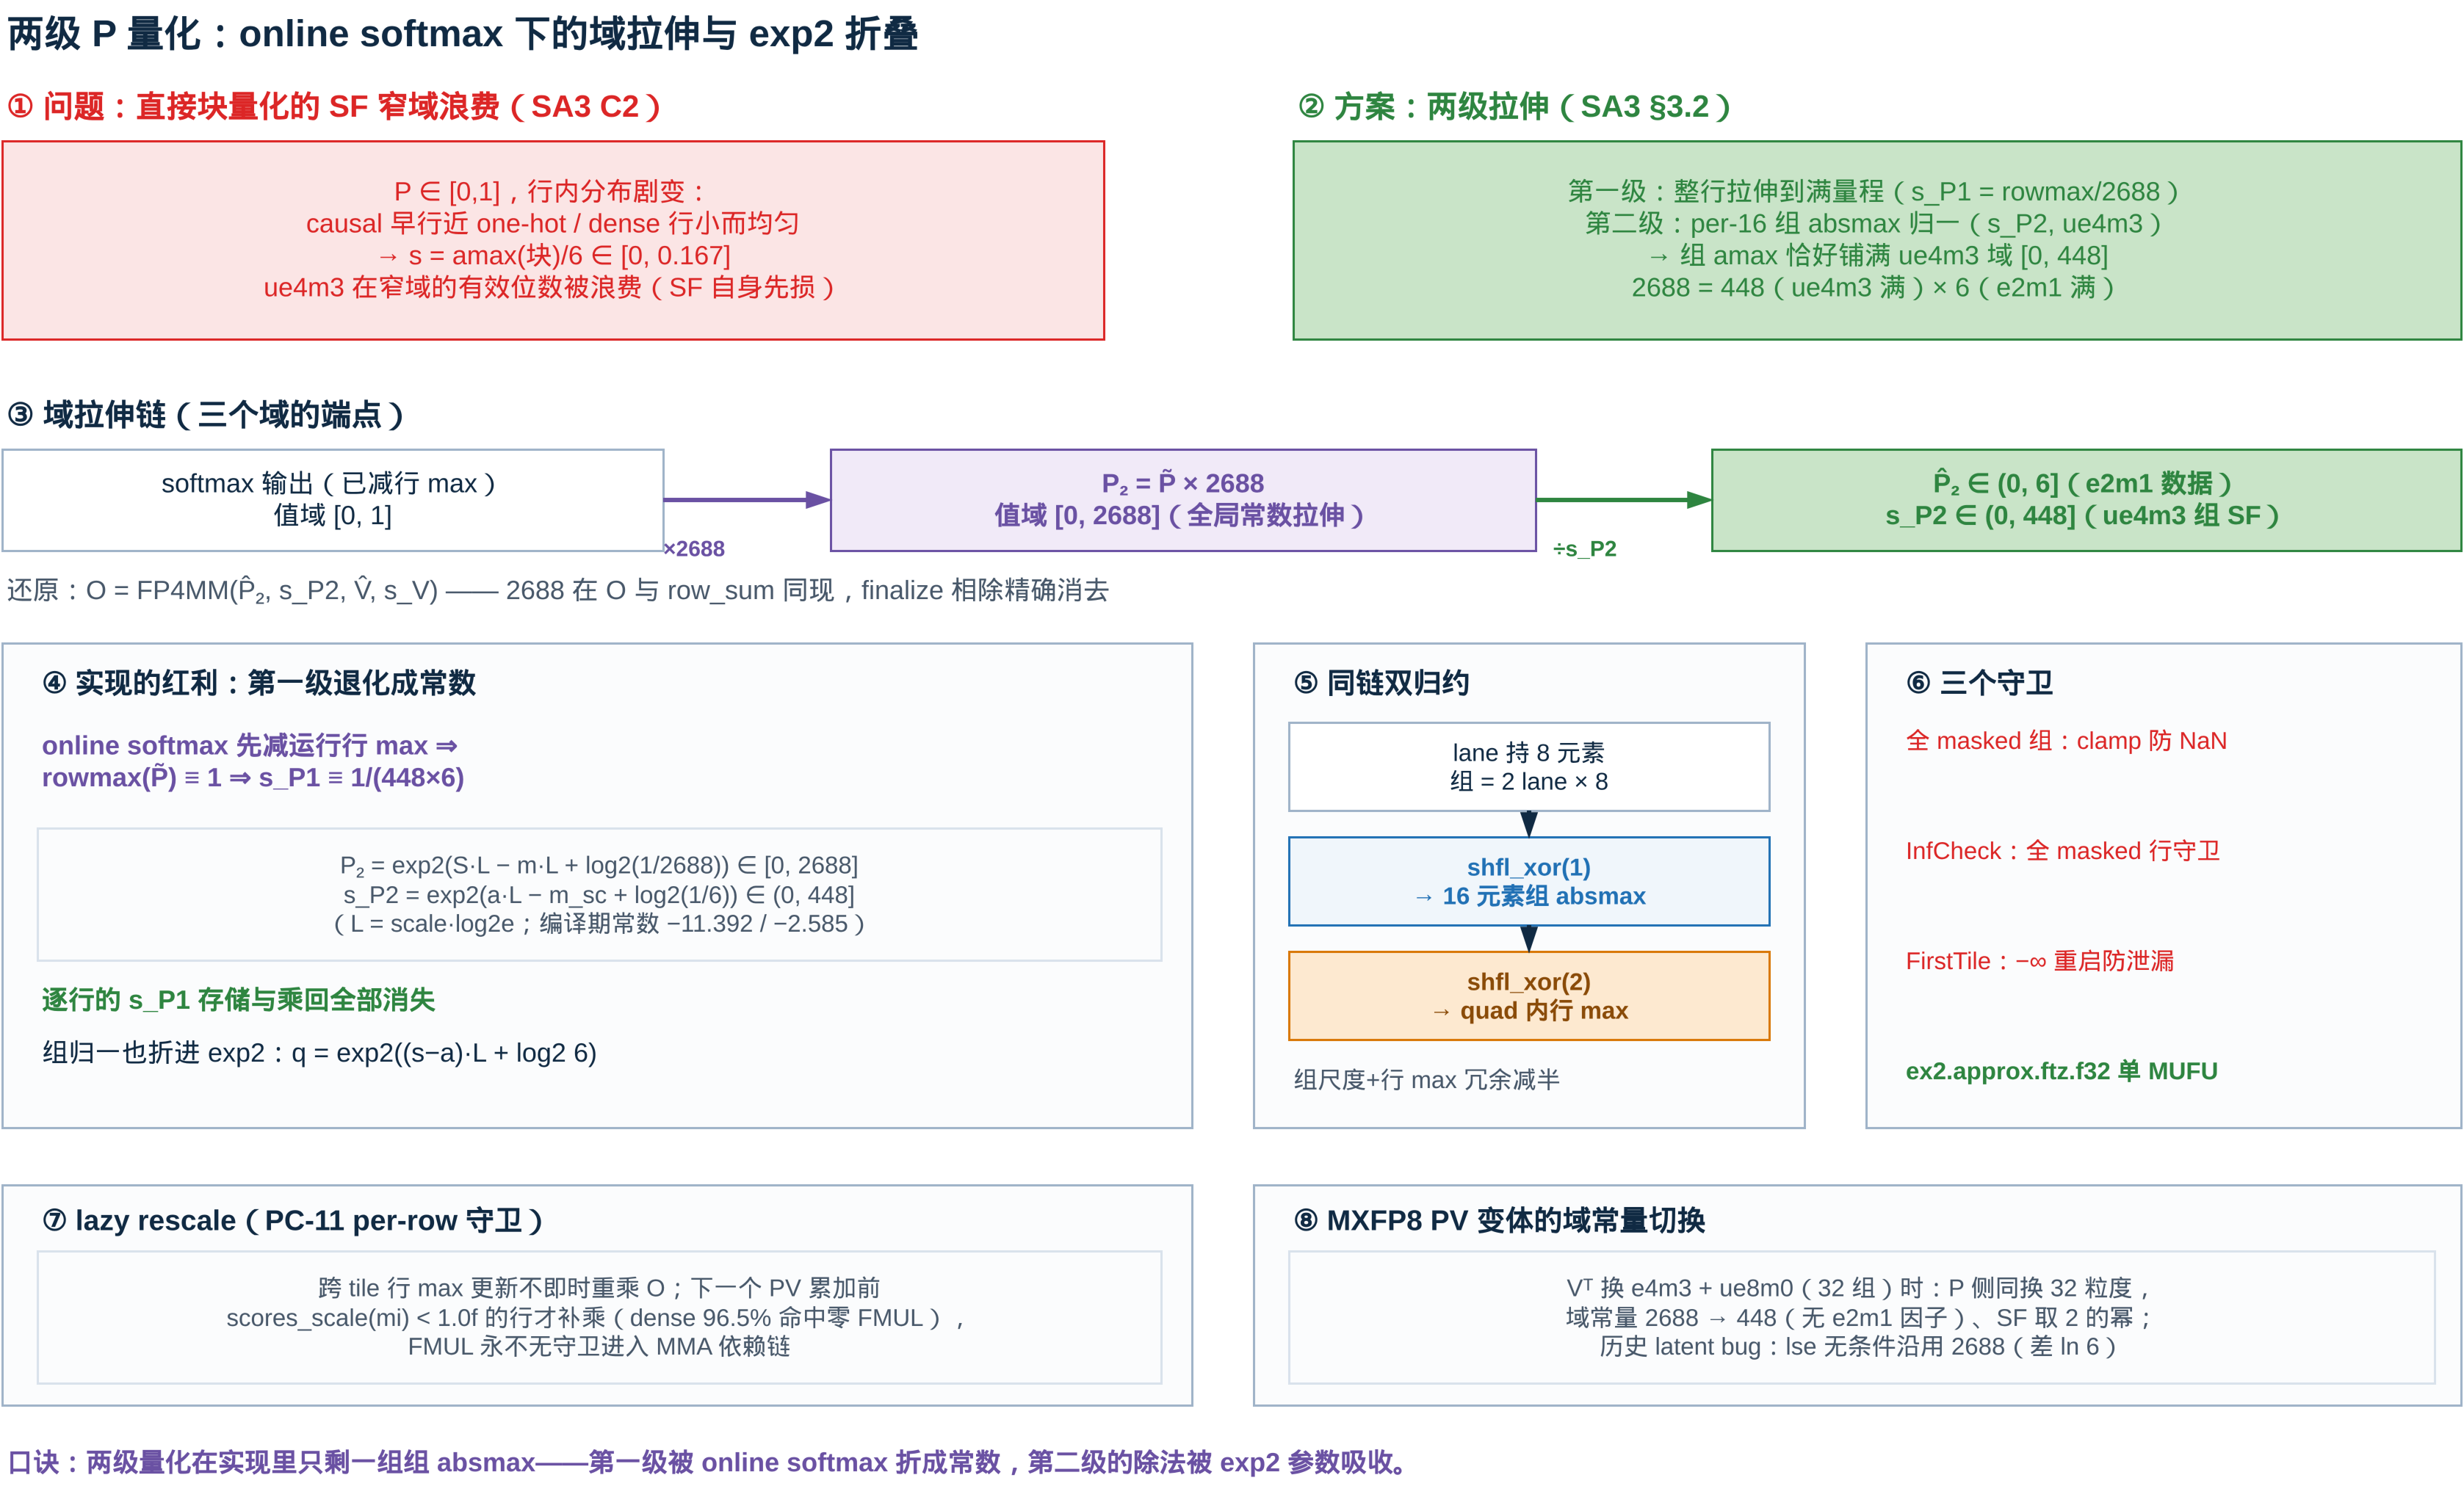
\includegraphics[width=0.98\textwidth]{figures/fig-32-1-two-level-p.png}
  \caption{两级 P 量化的域拉伸：online softmax 使第一级退化为全局常数
  $1/2688$ 并折进 exp2 shift；第二级 per-16 组 absmax 铺满 ue4m3 域，
  组归一化同样折进 exp2 参数。}
\end{figure}

\begin{figure}[H]
  \centering
  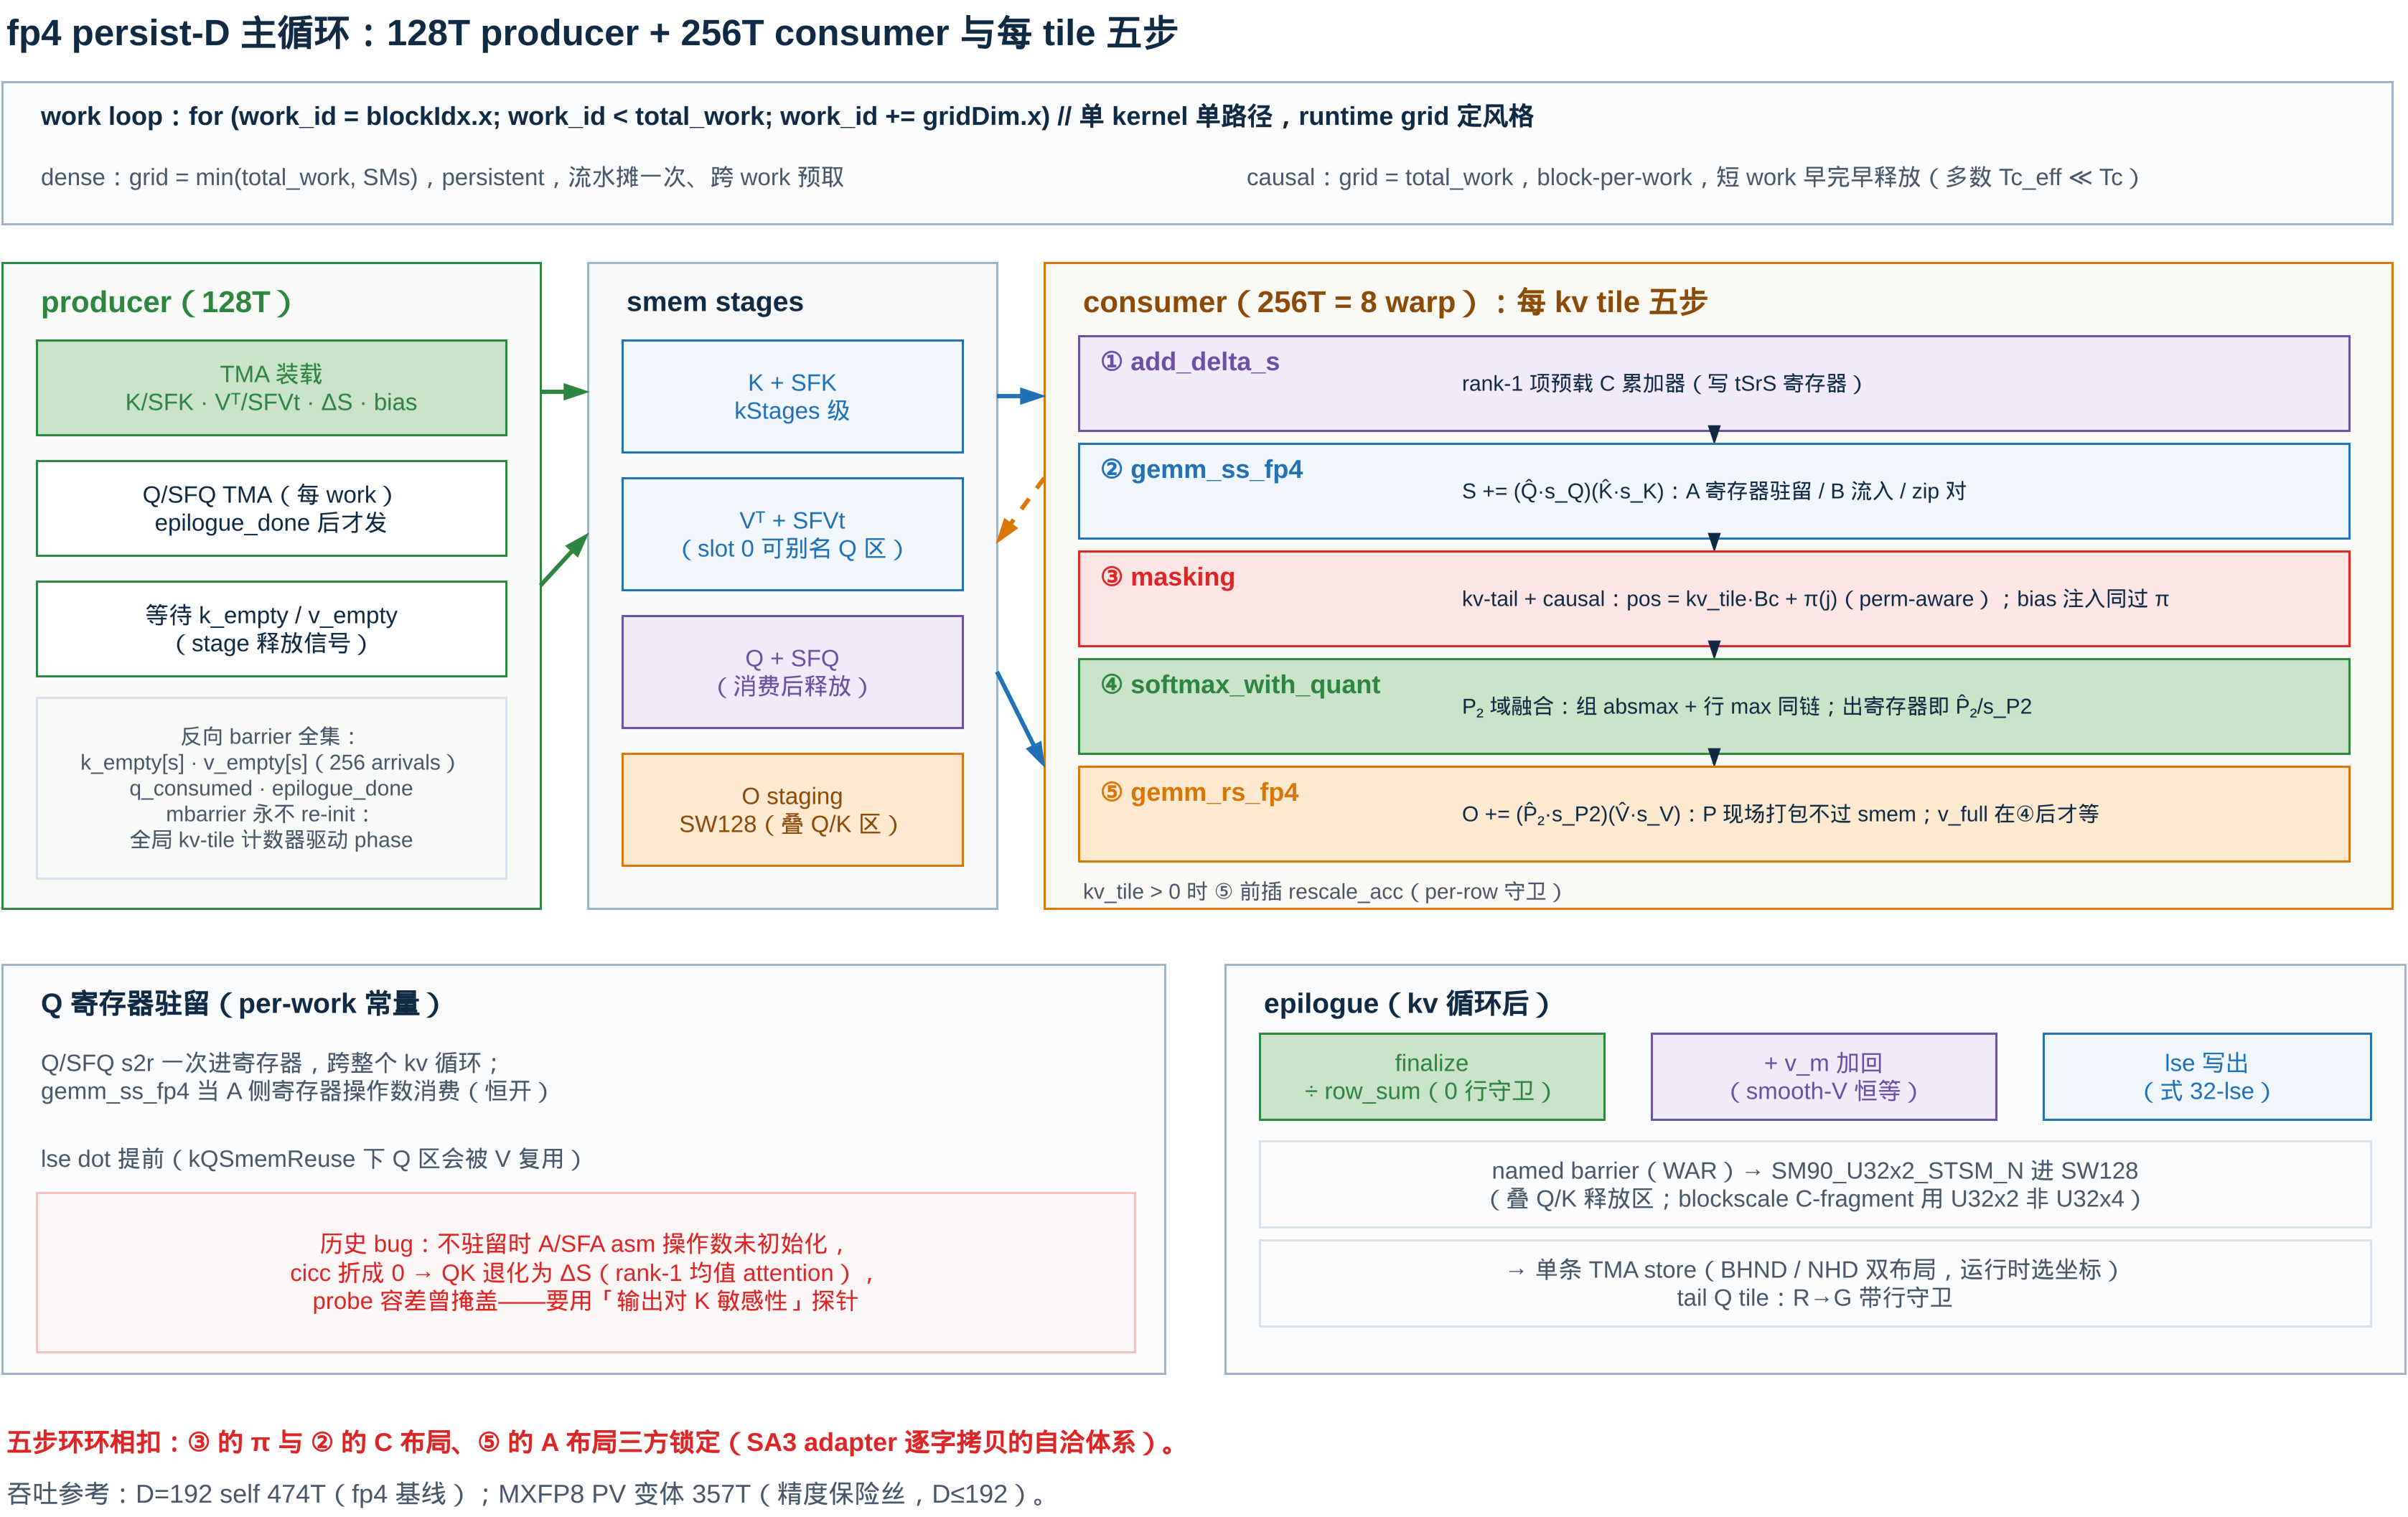
\includegraphics[width=0.98\textwidth]{figures/fig-32-2-persist-d-loop.png}
  \caption{fp4 persist-D 主循环数据流（128T producer + 256T consumer）：
  每 kv tile 的五步（$\Delta S$ 预载 $\to$ QK $\to$ masking $\to$ 融合
  softmax/P 量化 $\to$ PV），barrier 永不 re-init，grid 由 runtime 定
  persistent 或 block-per-work。}
\end{figure}

\section{性能分析}

\subsection{本机 e2e（fp4 vs SDPA）}

表~\ref{tab:32-mxfp8} 汇总 \texttt{--fp4-pv-mm-type fp8} 变体（数据落
盘 \texttt{.tmp/book-bench/ch32/}）；fp4 基线表见
第~\ref{ch:31}~章表 31.2（self 1.49--2.11x、causal 1.23--1.61x，
16 格全绿）。

\begin{table}[H]
  \centering
  \caption{MXFP8 PV 变体 vs fp4 基线（PRO 5000，$B{=}1,H{=}32,N{=}8192$，
  fp16 口径，allclose 全绿）}
  \label{tab:32-mxfp8}
  \begin{tabular}{@{}rlllll@{}}
    \toprule
    $D$ & mxfp8 self (ms) & vs fp4 & mxfp8 causal (ms) & vs fp4 & 加速比
    (self/causal) \\
    \midrule
    64  & 2.24 & $+39\%$ & 1.41 & $+31\%$ & 1.07x / 0.96x \\
    128 & 3.47 & $+38\%$ & 2.17 & $+30\%$ & 1.48x / 1.24x \\
    192 & 4.62 & $+33\%$ & 3.06 & $+28\%$ & 1.56x / 1.25x \\
    \bottomrule
  \end{tabular}
\end{table}

MXFP8 PV 付出 28--39\% 的代价：$V^\top$ 数据 8 bit 带宽翻倍、atom 换
\texttt{m16n8k128}，两者吞吐相近但带宽直接体现在 e2e。它的定位是
\textbf{精度保险丝}（$D\le192$ 的 smem 预算内），不是性能选项
（第~\ref{ch:31}~章 31.6 同结论）。

\subsection{fp4 对 fp8 的相对收益}

历史对照（RFC/skill 记录口径，非本机当日）：attn kernel 本身 fp4 比
fp8 快 $\sim$23\%——blockscale mxf4nvf4 吞吐与 fp8 dense 相当，收益
全部来自\textbf{带宽}（K/V/SF 字节减半以上）；D=192 的 e2e 比值
self 1.47x / causal 1.29x / gqa 1.50x。本机同日对照可复算：fp4
D=192 self 3.48ms（表 31.2）对 fp8 persist-D 同 shape 的表 29.2 数据。

\subsection{已落地与已证伪的微优化}

已落地：条件 rescale（PC-11 per-row 守卫，dense 96.5\% 命中，
-4.9\%；attn-mask 场景再 -3.7/-4.7\%）、\texttt{ex2.approx.ftz.f32}
（消 ptxas range 胶水，-5.9\%）、regalloc 按 D 门控（$D\le128$ 用
\texttt{alloc<224>}，$D\ge192$ 必须 232）。

已证伪（默认关闭/代码保留，勿重复）：Q smem 复用（fp4 的 L1TEX
sector hit 已 96.75\% 饱和，fp8 的前提不成立，实测 +1.8\% 回退，
\texttt{attn\_traits.cuh} L19--28 注释——与 fp8 章的同名机制结论相
反，很好的对照案例）；rescale merge in-place（把 FMUL 拉进 MMA 依赖
链，+1.7\%）；V/SFV 首块 s2r 提前藏进 softmax（PC-4：+1.3--1.7\% 净
负，LDSM 目的寄存器跨 softmax 链拉长 live-range；NCU 证实 B 供给非
瓶颈，wait 主体在 A 操作数串行链——persist-D 微优化到顶的标志）。

\section{实践经验}

\textbf{fragment adapter 是经验锁定的整体}。kv\_perm32、$\Delta S$
槽位算术、\texttt{LayoutP}/\texttt{LayoutSFP} 打包、$V^\top$ 转置存储
——SA3 的这套 adapter 相互补偿、自洽成体系（头注释 L25--37：empirical
lock 在 \texttt{.tmp} 的对齐探针里逐项验证过，dense e2e 与 dequant 仿真
一致）。逐字拷贝 + 只修 masking 是正确的移植姿势；单独「改进」其中
一环会破坏补偿关系。

\textbf{精度评估的口径}。e2m1 的 最坏 $\sim$25\% 的相对量化误差使 P/V 两级误差叠
加后 causal 尖峰行 max\_abs 天然 0.5--0.75（probe 仿真与 kernel 同
级，格式固有）；SA3 论文自身用 cosine 评估。工程验收看 mean\_abs
（0.014--0.03）与容差（dense 0.15 / causal 0.70），用 fp8 的容径卡
fp4 会全军覆没。hybrid（fp16 前 $n_{early}$ 行）是尖峰行的工程解法
（b0/b1 误差 2.6/0.99 $\to$ 0.000/0.001，剩余长尾由 V 量化主导）。

\section{常见坑}

\begin{enumerate}[itemsep=2pt,topsep=2pt]
  \item \textbf{masking 不 perm-aware}：causal 谓词按原始列 index 判
        定，$N{=}512$ max\_abs 3.3（上游 SA3 真实 bug；本章 32.4.3 的
        $pos$ 公式）。
  \item \textbf{mxfp8 域常量}：PV 换 mxfp8 后 lse 仍用 2688——差
        $\ln6$ 的 latent bug，按 \texttt{kPvMxfp8} 编译期分流域常量。
  \item \textbf{mbarrier re-init 是 UB}：跨 work 循环里对活跃 barrier
        re-initialize 行为未定义（PTX ISA 9.7.13.15.9），用全局 tile
        计数器驱动 phase。
  \item \textbf{stale AbsMaxP}：组 absmax 寄存器跨 tile/跨 work 复用，
        每 FirstTile 必须从 $-\infty$ 重新起步（L151--154 注释），
        否则上个 work 的尺度泄漏进当前行。
  \item \textbf{未初始化 asm 操作数被折叠}：Q 不驻留寄存器时 cicc 把
        A/SFA 操作数折成 0，QK 静默退化（32.4.2 的历史 bug）。
  \item \textbf{subbyte smem 指针}：e2m1 tensor 必须
        \texttt{make\_smem\_ptr}，裸 \texttt{reinterpret\_cast} 地址差
        2 倍、stage$\ge$1 TMA 越界（第~\ref{ch:31}~章 31.4.6）。
\end{enumerate}

\section{面试要点速查}

\begin{enumerate}[itemsep=2pt,topsep=2pt]
  \item 两级 P 量化：$s_{P1}=\mathrm{rowmax}/2688$、
        $\tilde P_2\in[0,2688]$、$s_{P2}$ per-16 组 ue4m3；2688 =
        448（ue4m3 满）$\times$ 6（e2m1 满）。
  \item online softmax 的退化红利：行 max 恒 1 $\Rightarrow$ 第一级变
        全局常数折进 exp2 shift——两级量化在实现里只剩一组 absmax。
  \item 组归一化折进 exp2 参数：$q=\exp_2((s-a)L+\log_2 6)$，rcp 与
        FMUL 段消失；row\_sum 用 FMA 吸收 $s_{P2}$。
  \item 2688 的消去：$O$ 与 row\_sum 同带常数，finalize 相除精确抵消。
  \item dense persistent / causal block-per-work：单 kernel 单路径，
        runtime grid 定风格；barrier phase 由全局 tile 计数器驱动。
  \item blockscale QK/PV 的 A 侧差异：Q 寄存器驻留（per-work 常量）、
        P 寄存器现场打包（quantize\_and\_pack\_p），B 侧才走 smem
        stage。
  \item fp4 vs fp8 的收益来源：MMA 吞吐持平、带宽减半——memory-bound
        attention 的收益逻辑。
\end{enumerate}

\section{最小测试与动手实验}

\begin{lstlisting}[style=console]
export CUDA_VISIBLE_DEVICES=7 FFPA_CUDA_ALLOW_SMALL_D=1
python -m ffpa_attn.bench --fwd-backend cuda --cuda-impl fp4 \
  --tasks self-attn causal --D 192 --no-bwd --show-allclose
# MXFP8 PV（精度保险丝，D<=192）：
python -m ffpa_attn.bench --fwd-backend cuda --cuda-impl fp4 \
  --tasks self-attn causal --D 192 --no-bwd --show-allclose \
  --fp4-pv-mm-type fp8
\end{lstlisting}

\begin{enumerate}[itemsep=2pt,topsep=2pt]
  \item \textbf{两级域验证}：读 \texttt{fp4\_pscale.cuh} L117--128 的
        三个编译期常数，手推
        式~\ref{eq:32-p2-domain} 的两个值域端点（$P_2=2688$ 当
        $s=m$；$s_{P2}=448$ 当组 absmax $=$ 行 max）。
  \item \textbf{mxfp8 A/B}：复现表~\ref{tab:32-mxfp8} 的三档 D，验证
        $D{=}256$ 被 traits 的 smem 断言拒绝。
  \item \textbf{causal 风格对照}：读 \texttt{launch/cute\_fp4\_persist\_d.cuh} 的
        grid 选择（\texttt{causal ? total\_work : min(...)}），解释为
        什么 causal 的多数 work 选 block-per-work。
  \item \textbf{InfCheck 场景}：构造 $N_q>N_{kv}$ 的 cross 输入跑
        causal，确认左上角全 masked 行的 lse/O 有限（无 NaN）。
\end{enumerate}

\section*{延伸阅读}
\addcontentsline{toc}{section}{延伸阅读}

\begin{itemize}[itemsep=0pt,topsep=2pt]
  \item \texttt{cute/fp4/sm\_120/persist\_d.cuh} 头注释（L1--55）：
        数学链、列对齐锁定、两级 P、subbyte；
  \item \texttt{cute/fp4/fp4\_pscale.cuh} L117--195：融合 softmax 的
        域折叠与 shuffle 链；
  \item \texttt{cute/fp4/fp4\_gemm.cuh} L91--218：\texttt{gemm\_ss\_fp4}
        与 \texttt{gemm\_rs\_fp4} 的流水与 barrier 协议；
  \item SageAttention3 论文 §3.2（两级量化）与 Algorithm 1（完整数值
        链）；sm\_120 split-D 与 M4N2 家族见第~\ref{ch:30}~章的 fp8
        同构实现。
\end{itemize}
